\documentclass[xcolor=dvipsnames]{beamer}

\usepackage{xcolor}
\usepackage[ngerman]{babel} % deutsche Silbentrennung
\usepackage[utf8]{inputenc} % wegen deutschen Umlauten
\usepackage{pdfpages}
\usepackage{graphicx}
\usepackage{pst-node}% http://ctan.org/pkg/pst-node

\usetheme{metropolis}           % Use metropolis theme
\title{The smallest grammar problem}
\date{05. Juli 2019}
\author{Edgar Dorausch}
%\institute{Centre for Modern Beamer Themes}
\begin{document}
\maketitle

\newcommand{\Gap}{$ $ \linebreak}
\newcommand{\FrameName}{
	\ifthenelse{\equal{\subsecname}{}}{
		\secname
	}{
		\secname \thinspace -\thinspace\subsecname
	}
}

\newcommand{\Fresh}{\ddagger}


\section{Motivation und Anwendung}

\begin{frame}{\FrameName}
	\begin{itemize}[<+->]
	%	\item \alert<4>{This is\only<4>{ really} important}
		\item pattern recognition
		\item compression
		\item Sprachstruktur
	\end{itemize}
\end{frame}

\section{Definitionen und Wiederholung}
\begin{frame}{\FrameName}
	\begin{block}{Kontextfreie Grammatik}
		\Gap
		Eine KFG ist ein Quadrupel $(\Sigma,\Gamma,S,\Delta)$ mit
		\begin{itemize}
			%	\item \alert<4>{This is\only<4>{ really} important}
			\item $\Sigma$ - Terminalalphabet
			\item $\Gamma$ - Nichtterminalalphabet
			\item $S$ - Startsymbol
			\item $\Delta$ - Menge von Regeln der Form $T\rightarrow\alpha$\linebreak
			$T \in \Gamma$;
			$\alpha \in (\Sigma \cup \Gamma)^\ast$
		\end{itemize}
	\end{block}
	
\end{frame}

\begin{frame}{\FrameName}
\begin{alert}{Besonderheit!:}
	\Gap
	Die Grammatiken sollen nur ein Wort erzeugen. Deshalb:
	\begin{itemize}
		
		\item Grammatik muss azyklisch sein
		\item Für jedes $T \in \Gamma$ existiert nur eine Regel in $\Delta$
	\end{itemize}
\end{alert}
\end{frame}

\begin{frame}{\FrameName}
\begin{block}{Expansion  eines Strings $\alpha$}
	\Gap
	Erhält man durch erschöpfendes Anwenden der Regeln in einer Grammatik bis nur noch Terminale enthalten sind. \linebreak
	Notation: $\langle \alpha \rangle$
\end{block}
\end{frame}

\begin{frame}{\FrameName}
\begin{block}{Expansionslänge}
	\Gap
	Anzahl der Zeichen in der Expansion eines Strings $\alpha$ \linebreak
	Notation: $[\alpha]  = \lvert \langle \alpha \rangle \lvert$
\end{block}
\end{frame}

\begin{frame}{\FrameName}
\begin{block}{Größe einer Grammatik G}
	\Gap
	Anzahl der Zeichen in den rechten Seiten der Grammatikregeln\linebreak
	Notation: $m = \lvert G \lvert = \sum\limits_{(T \rightarrow \alpha) \in \Delta} \langle \alpha \rangle$ \linebreak $ $\linebreak
	Größe der kleinsten Gramatik für einen String: $m^*$
\end{block}
\end{frame}

\begin{frame}{\FrameName}
\begin{block}{Beispiel}
	$$
	G \colon \begin{Bmatrix} 
		S \rightarrow rhaTber \textvisiblespace TTa \\
		T \rightarrow bar
	\end{Bmatrix}
	$$
	
	$\langle S \rangle = rhabarber \textvisiblespace barbara$ \linebreak
	$[S] = 17$ \linebreak
	$\lvert G \lvert = 11$
\end{block}
\end{frame}

\begin{frame}{\FrameName}
\begin{block}{Approximation Ratio}
	\Gap
	Sei $G_A$ die Grammatik, die von einem Algorithmus $A$ erzeugt wird.
	$$
	a(n) = \alert<2>{\max\limits_{\alpha \in \Sigma^n}}\frac{
		\textrm{$\lvert G_A \lvert$ für $\alpha$}
	}{
		\textrm{$m^*$ für $\alpha$}
	}
	$$
	\begin{center}\alert{
			
			\only<2>{Worstcase!}
		}
	\end{center}
	
\end{block}
\end{frame}

\begin{frame}{\FrameName}
\begin{table}
	\caption{Landau Notation}
	\begin{tabular}{ r p{3.5cm} l}
		
		$f \in o(g)$ & "$f < g$" \\
		%$\only<1>{f \in \mathcal{O}(g)}\only<2>{\alert{f \in \mathcal{O}(g)}}$ & "$f\leq g$" \\
		\textcolor{gray}{(Upper bound)} $f \in \mathcal{O}(g)$ & "$f\leq g$" \\
		$f \in \Theta(g)$ & "$f = g$"\\
		\textcolor{gray}{(Lower bound)} $f \in \Omega(g)$ & "$f \geq g$"\\
		$f \in \omega(g)$ & "$f > g$"\\
	\end{tabular}
\end{table}
\end{frame}

\section{Komplexität}
	
\begin{frame}{\FrameName}
\begin{itemize}[<+->]
	\item Vertex Cover lässt sich auf SGP reduzieren
	\item Zusammenhang mit Addition Chains \textcolor{gray}{(nicht im Vortrag)}
\end{itemize}
\end{frame}

\begin{frame}{\FrameName}
\begin{block}{Vertex Cover}
	\Gap
	Suche (minimale) Menge von Knoten, sodass jede Kante mindestens einen dieser Knoten enthält.\linebreak
	$ $\linebreak
	
	\only<1>{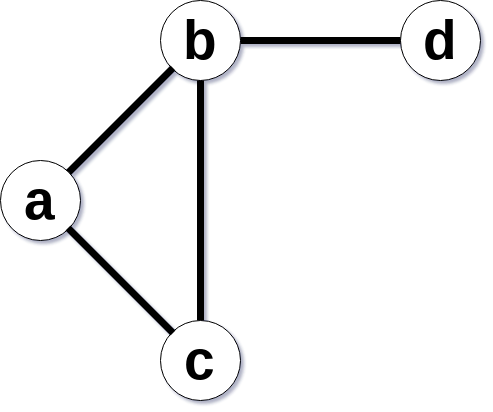
\includegraphics[width=0.25\textwidth]{Images/VertexCover/blank}}
	\only<2>{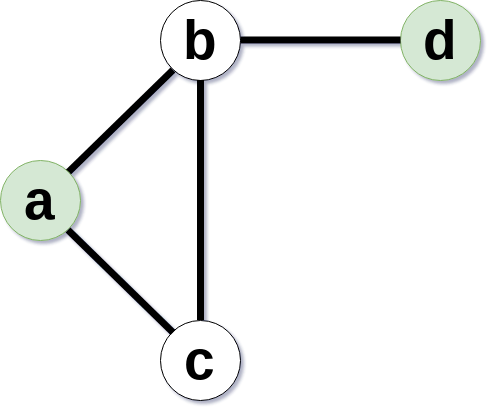
\includegraphics[width=0.25\textwidth]{Images/VertexCover/wrong}}
	\only<3>{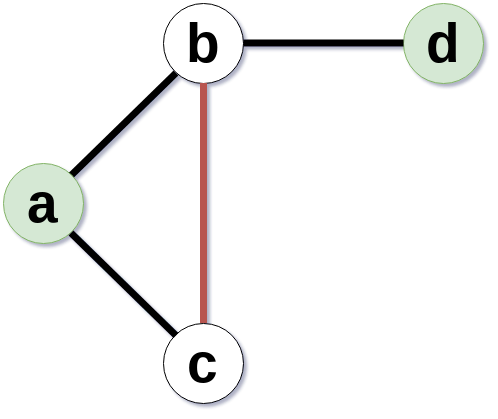
\includegraphics[width=0.25\textwidth]{Images/VertexCover/wrongMarked} \alert{(Kein Vertex Cover!)}}
	\only<4>{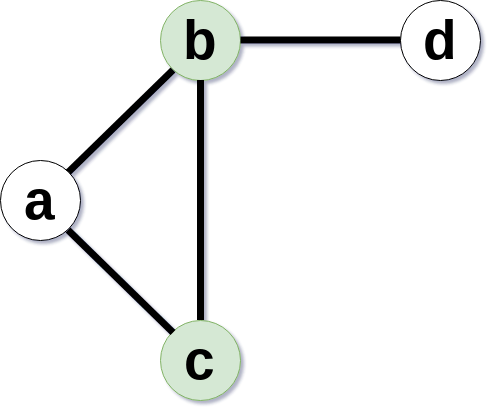
\includegraphics[width=0.25\textwidth]{Images/VertexCover/right}}
\end{block}
\end{frame}

\newcommand{\ExampleGraphV}{V = \{a,b,c,d\}}
\newcommand{\ExampleGraphE}{E = 
	\begin{Bmatrix}
		\{a,b\},
		\{a,c\},
		\{b,c\},
		\{b,d\}
	\end{Bmatrix}
}

\begin{frame}{\FrameName}
\begin{block}{Vertex Cover}
	\Gap
	$$\ExampleGraphV$$ 
	$$\ExampleGraphE$$
	\begin{center}
		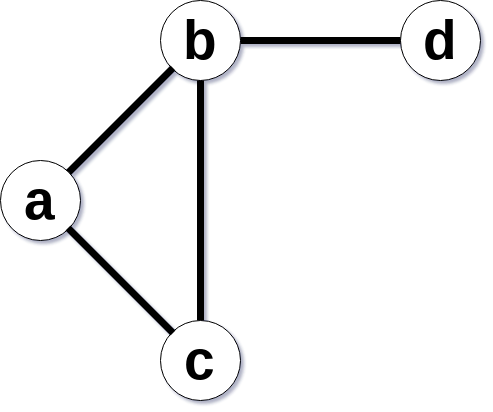
\includegraphics[width=0.35\textwidth]{Images/VertexCover/blank}
	\end{center}
\end{block}
\end{frame}

\newcommand{\ProdRuleOne}[1]{(\# #1 \Fresh #1\#  \Fresh )^2}
\newcommand{\ProdRuleTwo}[1]{\# #1 \#  \Fresh}
\newcommand{\ProdRuleThree}[2]{\# #1 \# #2\#  \Fresh}

\begin{frame}{\FrameName}
\begin{block}{Vertex Cover}
	\Gap
	$
	\alpha =
	\textcolor{OrangeRed}{
		\prod\limits_{v_i \in V}\ProdRuleOne{v_i}}
	\textcolor{PineGreen}{
		\prod\limits_{v_i \in V}(\ProdRuleTwo{v_i})}
	\textcolor{RoyalBlue}{
			\prod\limits_{\{v_i,v_j\} \in E}(\ProdRuleThree{v_i}{v_j})}
	$

	\newcommand{\PhantomAlpha}{\phantom{\alpha_{Beispiel} = (}}
	\newcommand{\ReductionExample}{
		\Gap
		$\ExampleGraphV; \ExampleGraphE$ \newline
		\Gap
		$
			\alpha_{Beispiel} =
			\textcolor{OrangeRed}{
				\foreach \n in {a,b,c,d}{\ProdRuleOne{\n}}
			} \linebreak
			\PhantomAlpha
			\textcolor{PineGreen}{
				\foreach \n in {a,b,c,d}{\ProdRuleTwo{\n}}
			} \linebreak
			\PhantomAlpha
			\textcolor{RoyalBlue}{
				\ProdRuleThree{a}{b}
				\ProdRuleThree{a}{c}
				\ProdRuleThree{b}{c}
				\ProdRuleThree{b}{d}
			} \linebreak
		$
	}

	% \only<1>{\phantom{\ReductionExample}}
	\only<2>{\ReductionExample}

\end{block}
\end{frame}




\section{Algorithmen}

\subsection{Vorüberlegungen}

\newcommand{\LowerBound}{\textcolor{TealBlue}{f_l(n)}}
\newcommand{\UpperBound}{\textcolor{Salmon}{f_u(n)}}

\begin{frame}{\FrameName}
\begin{block}{Lower bound bestimmen}
	\begin{itemize}[<+->]
		\item Definiere $\alpha$ \textcolor{gray}{(n = $|\alpha |$)}
		\item Bestimme lower bound von $m$ \linebreak \textcolor{gray}{$m \in \Omega(\LowerBound)$}
		\item Bestimme upper bound von $m^*$ \linebreak \textcolor{gray}{$m^* \in \mathcal{O}(\UpperBound)$}
	\end{itemize}
	\only<4>{
		$\Rightarrow$
		\fbox{
		$a(n) \in \Omega(\frac{
			\LowerBound
		}{
			\UpperBound
		})$
		}}
\end{block}
\end{frame}

\subsection{LZ78}

\begin{frame}{\FrameName}
	\begin{block}{LZ78}
	
\end{block}
\end{frame}



\begin{frame}{\FrameName}
	\only<1>{
		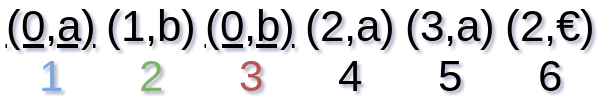
\includegraphics[width=\textwidth]{Images/LZ78/blank}}
	\only<2>{
		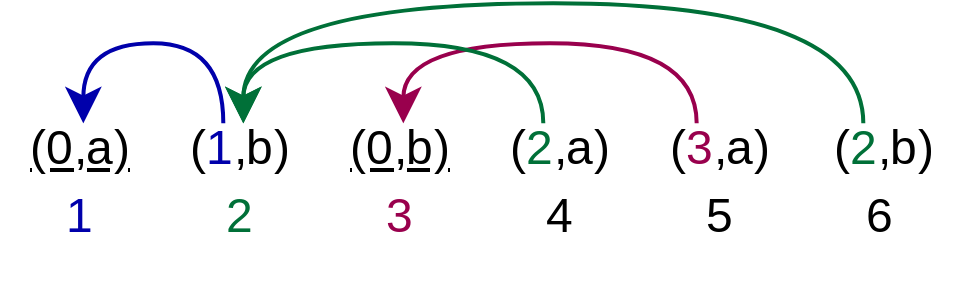
\includegraphics[width=\textwidth]{Images/LZ78/withRef}}
	\only<3>{
		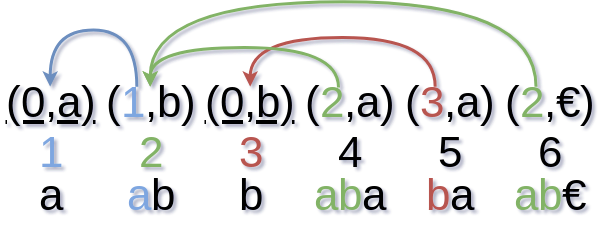
\includegraphics[width=\textwidth]{Images/LZ78/full}}
\end{frame}

\subsection{global algorithms}
\begin{frame}{\FrameName}
	\begin{block}{TODO}
	\Gap
	$a^2 + b^2 = c^2$
\end{block}
\end{frame}

\subsection{LZ77 variant}
\begin{frame}{\FrameName}
	\begin{block}{TODO}
	\Gap
	$a^2 + b^2 = r^2$
\end{block}
\end{frame}

\end{document}